\documentclass{article} 
\usepackage[utf8]{inputenc}
\makeatother\usepackage{graphicx} 
\usepackage{amsmath} 
\usepackage{amsfonts} %for \mathbb \newcommand{\indep}{\rotatebox[origin=c]{90}{$\models$}}
\usepackage [english]{babel}
%\usepackage [autostyle, english = american]{csquotes}
%\MakeOuterQuote{``}

\title{The Bayesian approach to family-wise error revisited}
\date{August 2016}
\begin{document}

\maketitle


\section{Abstract}

Statistical errors accumulate whenever one estimates or tests multiple unknowns from data, as is common in biological imaging and -omics. One conventional frequentist solution seeks to limit the aggregate error over all tests, notably the ``family-wise'' error. An alternative solution, which is closely tied to Bayesian hierarchical models, is to control the error associated with parameter estimation, rather than parameter testing. To better compare these approaches, we define a Bayesian family-wise error. We evaluate this error for the popular hiearchical linear model, and show that it is much smaller at any given test threshold under the family null hypothesis. Our results build on previous work on the Bayesian False Discovery Rate.

\section{Introduction}

Statistical methods often aim to identify some parameter or signal $u$, such as the reliable causal effect of an experimental manipulation, despite unexplained variation or ``noise'' in the data. Because of this noise, inference on $u$ varies randomly over seemingly identical measurement conditions, which exhagerates or ``overfits'' the estimated magnitude $u$. This problem grows with the dimensionality of the inference, for example when $u \equiv \{u_i: i \in I \}$ is a large collection of unknown conditions/voxels/genes/time-points with index set $I$. This is because noise can separately corrupt each estimated component $u_i$. When we test many hypotheses concerning the individual elements of $u$ this overfitting is known as the multiple testing problem. There are therefore different ways to quantify this overfitting/overtesting problem and different ways to contain the problem by reducing the impact of noise on inference. All these corrections must balance overfitting and underfitting.

Statistical methods often aim to identify some parameter or signal $u$, such as the reliable causal effect of an experimental manipulation, despite unexplained variation or ``noise'' in the data. Because of this noise, inference on $u$ varies randomly over seemingly identical measurement conditions, which exhagerates or ``overfits'' the estimated magnitude $u$. This problem grows with the dimensionality of the inference, for example when $u \equiv \{u_i: i \in I \}$ is a large collection of unknown conditions/voxels/genes/time-points with index set $I$. This is because noise can separately corrupt each estimated component $u_i$. When we test many hypotheses concerning the individual elements of $u$ this overfitting is known as the multiple testing problem. There are therefore different ways to quantify this problem and to fix. The challenge for every solution is avoid over-correction or underfitting.

Conventional hypothesis testing procedures seek this balance by underfiting, favoring some null constraint on parameters such as $u_i=u_j$, unless this is can be falsified by a statistical test. Hierarchical Bayesian procedures achieve this balance through infered  probabilistic (distributional) constraints on $u$, not through deterministic constraints like $u_i=u_j$ above, see ``Bayesian and frequentist inference''. This rests on the additional assumption that unobserved signal $u$ was the outcome of some hidden random process, denoted $U$. For example, assuming hidden $u_i$ were randomly sampled from an identical, low variance populatian is akin to a null hypothesis $u_i \approx u_j$ (because it is improbable that they differ from each other by much). Under this ``null'' prior assumption, Bayes theorem automatically shrinks the posterior estimates $u_i-u_j$ toward zero, which mirrors the bias for retaining the null hypothesis in the conventional approach discussed above. (This is akin to constraining the norm $|u|$). As above, this conveniently suppresses spurious inferences due to noise without needing a hypothesis test to filter them out, but risks underfitting whenever our premise is wrong. Importantly then, hierarchical shrinkage or ``regularization'' is calibrated according to the data itself, by learning the latent generating process for $u$  or, more coloquically, ``learning the prior''. This process can be intui- tively interpreted as learning the cross-gene heterogeneity from the data. Learning enables us to balance undercorrection or overcorrection\footnote{Hierarchical methods thus automatically balance underfitting and overfitting in a principled way, without appealing to the arbitrary $0.05\%$ convention to select a test threshold. Instead, this balance depends on a learned probability model of the latent random process which generated $u$. Shrinkage increases to counter overfitting whenever the null random process is deemed plausible, otherwise it decreases, to avoid unnecessary underfitting or overshrinking.}.

Conventional hypothesis testing procedures seek to avoid overfitting by constraining the number of free parameters, adopting some default null hypotheses such as $u_i=u_j$. This solution involves setting a high threshold for rejecting the default null, so naturally has little sensitivity to detect small, but non-zero $u_i-u_j$\footnote{The insensitivity - or ``type-II'' error - is the unavoidable cost of prioritizing ``type-I''  or ``false-positive'' erro. In general, there is always a tradeoff between type-II for type-I, underfitting and overfitting. This relates to the famous bias-variance tradeoff. The type-II probability quantifies the test's conservative bias: accepting the default constraint $u_i=u_j$  introduces possible bias (whenever $u_i \neq u_j$) in return for reducing error variance (equating parameters $u_i=u_j$ means we can pool data across conditions to estimate just one unknown, thereby benefiting from the law of large numbers to reduce variance).}. To control \textit{aggregate} type-I over multiple tests we must increase the test threshold, so this insensitivity grows. By collapsing small differences to the default null hypothesis with increasingly high probability in this way, this conventional approach anticipates more recent hierachical shrinkage methods, as discussed below.

Hierarchical Bayesians address the overfitting problem through probabilistic (distributional) constraints on $u$, not through deterministic constraints like $u_i=u_j$ above, see ``Bayesian and frequentist inference''. This rests on the additional assumption that unobserved signal $u$ was the outcome of some hidden random process, denoted $U$. For example, assuming hidden $u_i$ were randomly sampled from an identical, low variance populatian is akin to a null hypothesis $u_i \approx u_j$ (because it is improbable that they differ from each other by much). Under this ``null'' prior assumption, Bayes theorem automatically shrinks the posterior estimates $u_i-u_j$ toward zero, which mirrors the bias for retaining the null hypothesis in the conventional approach discussed above. (This is akin to constraining the norm $|u|$). As above, this conveniently suppresses spurious inferences due to noise without needing a hypothesis test to filter them out, but risks underfitting whenever our premise is wrong. Importantly then, hierarchical shrinkage or ``regularization'' is calibrated according to the data itself, by learning the latent generating process for $u$  or, more coloquically, ``learning the prior''. This process can be intui- tively interpreted as learning the cross-gene heterogeneity from the data. Learning enables us to balance undercorrection or overcorrection\footnote{Hierarchical methods thus automatically balance underfitting and overfitting in a principled way, without appealing to the arbitrary $0.05\%$ convention to select a test threshold. Instead, this balance depends on a learned probability model of the latent random process which generated $u$. Shrinkage increases to counter overfitting whenever the null random process is deemed plausible, otherwise it decreases, to avoid unnecessary underfitting or overshrinking.}.

To compare frequentist and Bayesian solutions more formally we study their family-wise errors assuming data generated under the family null hypothesis $u_i = 0$ for all $i \in I$. This family null hypothesis models the scenario when there is no signal anywhere in $u$, and implies for example $u_i=u_j=0$ for all $i \neq j$, and $u_{max}=0$. In this scenario, frequentist inference procedures commit a family-wise error whenever the frequentist maxima exceeds test threshold $h>0$, because this means falsely concluding there is one or more positive effect, see ``Classical maxima and conventional control''. Critically, we note that Bayesian procedures also incur a family-wise error when the \textit{posterior maxima} of a hierarchical Bayesian model exceeds $h$: this error is equivalent to falsely believing one or more elements of $u$ have positive signal, given  data generated under the family null\footnote{The posterior maxima is just the credible magnitude of the maximal effect, which is $0$ by definition in family null data. We emphasize that the distribution of the posterior maxima is \textit{not} the familiar maxima of the posterior distribution, i.e. not to the maximum \textit{a posteriori} or MAP estimate. Neither does it report posterior belief about which specific index (indices) take value $u_{max}$, for example it is not the distribution of the index with the largest marginal exceedence probability. For clarification on different types of maxima, see Appendix 2.}. This insight offers a conceptual bridge for us to compare Bayesian and frequentist family-wise probabilities, despite their different semantics and assumptions. In particular, we can ask which has a lower family wise error probability at a given threshold $h$. We have chosen to study the maxima because it is applicable across the very different hierarchical and frequentist models used in practice: spatial, cross-sectional, temporal, neither or both. For example, the posterior maxima is defined whether a discretely indexed, exchangeable random process, or a continuously-indexed, non-stationary process. Regularization of the maxima. 


From leadership paper: The error term U, which is an unobserved latent variable must not be confused with the residual term, which is the difference between the predicted and the observed value of y . This residual term is orthogonal to the regressors regardless of whether the error term is or not.

The probability of observing a table at least as extreme as the observed table, which is the sum of the probabilities of all the extreme tables (think Fishers exact, also the 2x2 confusion matrix?, but actually don't observe the whole table in that case).

y studies are affected by random-noise sources that naturally fall into a hierarchy, such as the biological variation among animals, tissues and cells, or technical variation such as measurement error. With a nested approach, the variation introduced at each hierarchy layer is assessed relative to the layer below it. We can use the relative noise contribution of each layer to optimally allocate experimental resources using nested analysis of variance (ANOVA), which generally addresses replication and blocking, previously discussed ad hoc.
Asymptotia is an assumption, as is 
,
Corrective penalties control the size of estimation or test errors. Bayesian ``penalize'' inferences incongruent with prior knowledge of the \textit{data-generating process}. Every prior is the posterior for some other analysis, which is a way to understand priors. Generating process is a story. Theorists model domain-speciific data generating processes. Conditional on the truth of that model, probability theory (Bayesian) \textit{determines} how to extract information about the process unknowns from the data, the unique posterior. To compare candidate generating models, simply compare the relative number of possible ways that each could have generated the observed data: this is the posterior plausibility. Sensitivity of small changes in the data story make big difference? Likelihood: if you want know something, condition on it. Assume you knew it and derive prediction on observables. 

Another solution to the high-dimensionality of the problem is the use of hierarchical Bayesian or penalized regression, which constrains the magnitude of the regression coefficients, and allows them to be estimated. LASSO and Ridge are most popular. LASSO is sparse estimator, meaning that it sets some regression coefficients to zero, while keeping others non-zero. (In a Bayesian setting, double exponential - which may overshrink due to light tails of double exponential and therefore introduce unnecessary bias- Generalized Double Pareto (GDP) prior to induce sparsity in a Bayesian Generalized Linear Model (GLM) setting (Madahian et al).) Ridge regression penalizes the sum of squared regression coefficients, but it does not reduce the number of parameters in the model. 
In Abraham et al. (2013) it has been shown in the context of GWAS that penalization decreases the false positive rate and increases the probability of detecting the causal SNPs.
The dimension and complexity of high-throughput gene expression data create many challenges.
Sparse Bayesian Generalized Linear Model.

Although it is appealing to introduce bias in small coefficients to reduce the mean squared error and model complexity, it is also desirable to limit the shrinkage of large coefficients 
Inverse problem (physical sciences) is an identifiability problem (statistics), so falsifiability is not possible. Identifiability necessary to distingish different process theories. Accept the null is naughty, from the modes tollens (Popperistic falsification) perspective, cf. Black swan, but this is a discrete hypothesis, c.f. the proportion of black swans. ``The continuous version of discrete logic is Bayesian inference''. 
Although the probability that the observed variance significantly deviates from the true variance is small for each individual gene, in a genomic study with many genes, the chance to encounter such deviants for some genes is high. The inflation of false positives during multiple testing issue is resolved by applying a stringent significance threshold.
 
Next, the top-level distribution is used to adjust the parameter estimate of every gene (Fig. 1e). If cross-gene heterogeneity is small, the adjustment will make the parameter esti- mates of different genes more similar to each other.
If the variability among genes is low relative to the sampling variability within a gene, the mean variance σ02 will receive a high weight. On the other hand, if the cross-gene variation is high compared to the within-gene sampling variability, more weight will be given to si2.
This weighted average technique to estimate the variance is called variance stabilization. It is widely used in analyses of gene expression microarrays4,8 and chromatin immunoprecipitation on til- ing microarrays (ChIP-chip)7 to detect dif- ferentially expressed genes and protein-DNA binding sites, respectively. Naturally, real microarray experiments are more complicated and contain more sources of variation than our example; thus, they can benefit from more sophisticated hierarchical models that capture those types of variation.

Aggregation of many small signals - c.f. small errors - over many dimensions: collective ``omnibus'' tests for increased power and reduced underfitting or type-II errors. 

The distribution of the Brownian Bridge maxima for gene set inference (``enrichment'').
Idea convert a finite sample into a continuous process (the sample cdf). Maximum deviation from zero measures collective differential expression of a prior gene set (the ``enrichment score''). Non-parametric Bridge maximum distribution under some hypothesis: null assumption of exchangeable class labels/values (of the discrete predictor) warrants their permutation.

Constrain nuissance parameters which are boring but important for target inferences: set them to a constant, equate across samples and pool (law or large numbers), relate them via a model of the random generative process. 

Several papers (Efron et al. 2000, Efron et al. 2001, Efron & Tibshirani 2002) connect empirical Bayes methods with false discovery rates.

 (Hereafter “FWE control” is always assumed to mean “in the strong sense.”)
$FWER = P[$at least one false positive among m hypothesis tests$]$
It is often of interest to assign uncertainties for inferring the true underlying regres- sion coefficients βj0 (j = 1,...,p) in the linear model (2). The classical concept of confidence intervals for single coefficients βj0 or confidence regions for a set G ⊆ {1, . . . , p} of coefficients {βj0; j ∈ G} can capture this. Somewhat easier is the case with statistical hypothesis testing for single or group hypotheses:
single: H0,j : βj0 = 0 versus HA,j : βj0 ̸= 0, (10) group: H0,G : βj0 =0∀j∈GversusHA,G : βj0 ̸=0foratleastonej∈G.(11)
These hypotheses are rather natural and often of major interest, namely for infer- ring whether a regression coefficient is zero (i.e., the corresponding covariate has no effect) or not.

higher power owing to improved weighting of the data.
places an upper bound on the statistical power
Methods that explicitly model population structure, family structure and cryptic relatedness are expected to perform better in the presence of these complexities than methods that do not
An assumption (e.g. of homogeneity) can easily be violated, and can lead to both type I and type II errors.

Formula (18) also allows for multiple testing adjustment among m tests, with respect to the familywise error rate (FWER) defined as

$FWER = P[$at least one false positive among m hypothesis tests$]$

When performing m hypothesis tests, it is important to adjust for multiplicity. If each of these m tests is performed at significance level α, it holds that FWER ≤ mα. This is due to the union bound but might be rather conservative in general. However, if the tests were independent, then FWER = (1 − (1 − α)m) ≈ mα which essentially achieves the upper bound. We can simply adjust the statistical tests by dividing the significance level by m or multiplying the corresponding p- values by m: this is known as the Bonferroni correction. However, for dependent tests, such a Bonferroni correction is overly conservative. When using the exact distribution in (18) one obtains much more powerful multiple testing adjustment for controlling the familywise error rate: this is essentially the Westfall-Young procedure [58] which has been shown to be optimal in certain settings [47]. Thus, multiple testing adjustment based on the simultaneous pivot as in (18) leads to a procedure which controls the familywise error rate and yet it has good power, particularly for settings with dependent tests and in comparison to a Bonferroni (or Bonferroni-Holm) multiple testing adjustment.
As we have seen above, simultaneous inference with respect to the sup-norm is a straightforward implication of Theorem 2.1 and (14). When looking at other norms such as the l2-norm, i.e.,

The family null is defined as $u_i=0$ for all $i \in I$. If we assume that $u_i$ are  independent mean zero random variables and common variance $\psi_U$, the family null now becomes simply $H_0: \psi_U = 0$ so that the dimension of $H_0$ does not depend on $|I|$ anymore.

Alternatives with small values of $\psi_U$ tend to have small values of $\sum_i u_i$.

``The Global Test tests the null hypothesis that the pathway is not associated with outcome labels. 

This null hypothesis only depends on the observed outcomes and on the genes in the pathway itself: the result is absolute, not relative to the other pathways.''

In the high-dimensional $(p>n)$ setting, testing for whether $X$ predicts outcome is equivalent to testing the hypothesis
$H_0 :u_1 = u_2 =···=u_{p} =0$
that all regression coefficients are zero. ``It is not possible to test this hypothesis in a classical way (with $u$ non-stochastic) because $p$ might be large relative to $n$. In this case there are too few degrees of freedom.''

``However, it is possible to test $H_0$ if it is assumed that $u_1, ..., u_p$ are a sample from some common distribution with expectation zero and variance $\tau_U$. Then a single unknown parameter $\tau_U$ determines how much the regression coefficients are allowed to deviate from zero. The null hypothesis becomes simply

$H_0: \tau_U = 0$''

This suggests a simple set-level fMRI test. Additionally, unlike previous authors (Goeman) who only offer ``diagnostics'' for why family null (``global'' hypothesis) was rejected, the hierarchical Bayesian methods can. 

``The model (1) with β random may be looked at in various ways. Firstly the distribution of β can be seen as a prior, with unknown shape and with a variance depending on an unknown parameter. Viewed in this way the model (1) is an empirical Bayesian model.
A second interpretation is to view the model as a penal- ized regression model, in which the estimated coefficients are shrunk towards a common mean. The log likelihood of Y can be written
loglik(Y , β ) = loglik(Y |β ) + loglik(β ),
where the first term on the right is the likelihood of the ordin- ary generalized linear model and the second term is known as the penalty. Well-known examples of penalized regres- sion include ridge regression (Hoerl and Kennard, 1970), which arises when β is normally distributed and the Lasso (Tibshirani, 1996), which is a variant where β has a double exponential distribution. Ridge regression with a logistic link function has been described by Le Cessie and Van Houwelingen (1992) and applied on microarray data by Eilers et al. (2001) with promising results.

he test in the next section. For this we write ri = j xij βj , i = 1, . . . , n. Then ri is the linear predictor, the total effect of all covariates for person i. Let r = (r1,...,rn), then r is a random vector with E(r) = 0 and Cov(r) = τ2XX′. The model (1) simplifies to''

Information criterea measure overfitting while regularizing priors reduce it (complementary).

locally most powerful test (score test) on the hyperparameter in an empirical Bayesian model (Goeman et al).

Typical multiple-testing procedure from microarray data analysis which uses the maximum of all absolute univariate T -statistics as a test statistic for the global null hypothesis (Goeman 2006)!!

empirical Bayes version of Neyman–Pearson lemma (Goeman 2006).

Multiple testing is used to infer sparse alternatives, ridge to infer others.

This type of testing procedure is often used in microarray data analysis. There are many variants, but the most basic form is the following: for i = 1,...,p a T -test statistic t i is calculated to test for association of each covariate with the outcome y. The test statistic ˜ T max = max.|t 1 |,...,|t p |/ is used to test whether there is an association between any covariate and y. The critical value of ˜ T max can be found either conservatively by using the Bonferroni adjustment or by using numerical methods.

    - If the fraction of variance of y explained by the design is low, the global test outperforms the test
that is based on the maximum absolute t-statistics of all covariates, a test which is designed to
find sparse alternatives [Goeman2006].
- We nonetheless consider this latter test here.

ANOVA inferences are only slightly affected by inequality of variance if the model contains only fixed factors and has equal or almost equal sample sizes. Alternatively, ANOVA models with random effects and/or unequal sample sizes could be substantially affected.
Fixed factor/parameter vs random factor/'parameter'. Hypothesis tests always rest on many untested simplifying model assumptions: Test of equal variance (hope to accept null), then test of equal mean (hope to reject null). Multiple comparisons of conditional mean and conditional variance! i.e. test whether a group-specific (factor combination) variances are equal. Levenes "homogeneity of variance" test (use Bartletts test if sure error is Gaussian).

In a second simulation experiment we look at sparse alternatives in high dimensional data.  We compare the power of the locally most powerful test with the power of the test that is based on T max , the maximum absolute t-statistic.

A complicating factor in this simulation is the lack of a simple and accurate method for find- ing the distribution function of the statistic T max , because of the dependence of the t-statistics.  We used simulation to find the α cut-off of T max for the design matrix X. The 0.05-cut-off was found at 0.062, using 20000 simulations of y under the null hypothesis. Note that this is only slightly below the crude Bonferroni corrected cut-off for p beta{ 1 2 , 1 2 .n − 1/} variables, which is at 0.064

The maximum absolute t-statistic of all covariates $\max|T_i|$  is designed to find sparse alternatives. (covariate = voxel?).
Testing  whether  there  is  a  predictive  effect  of  the  gene expressions on the clinical outcome is equivalent to testing the hypothesis $H_0: \beta_i=0$ or $H_0: \beta_1=...=\beta_p=0$. It is not possible to test this hypothesis in a classical way (with $\beta$ non-stochastic) because m might be large relative to n . In this case there are too few degrees of freedom. 

However,  it  is  possible  to  test H 0 if  it  is  assumed  that β 1 , ...  , β m are a sample from some common distribution with expectation zero and variance τ 2 . Then a single unknown para- meter τ 2 determines how much the regression coefficients are allowed to deviate from zero.  The null hypothesis becomes simply $\tau_0=0$.
Note that the choice of τ 2 I m (with I m the m × m identity mat- rix) as the covariance matrix of the stochastic vector β is not imperative. It is the most convenient choice which will yield a test that treats all genes on an equal footing. Any other m × m covariance matrix may be used to replace I m , if desired, result- ing in a different test with power against different alternatives.  For example a different diagonal matrix can be taken to reflect prior beliefs in the greater reliability of certain genes. Assum- ing positive correlations between the elements of β results in more power against alternatives where all β coefficients have the same sign. (JC, or a spatial process to dictate correlations.

However, when many groups of genes are to be tested, multiple testing procedures come back into play (Benjamini and Hochberg, 1995). Nested groups may be tested without adjustments to the α -level. Always keep in mind that groups of genes may never be chosen with reference to the  outcome 

If the fraction of variance of y explained by the covariates is low the test even outperforms the test that is based on the maximum absolute t-statistics of all covariates, a test which is designed to find sparse alternatives. 

restrictive assumptions.
 
Controlling the FWER has as an advantage that, if you choose to follow up only on a subset of the rejected set, maybe because of biological information or limited capacity, the FWER is also controlled for this subgroup. This so-called subsetting property is not guaranteed in an FDR setting, in which it can happen that the proportion of false positives in a chosen subset exceeds the chosen α-level. 


It is interesting to note that, whereas the emphasis in multiple testing procedures lies mainly on preventing type I errors, condoning the resulting type II errors, the lasso mostly focuses on including every potential “true” predictor, taking some additional ``noise variables'' more or less for granted. Again from a different perspective, this observation nicely illustrates the differences between the two approaches; for prediction purposes, in view of minimizing bias, it is better to include all true predictors with the risk of adding some extra noise variables whereas actually proving association asks for a more rigorous procedure.

Goeman and Solari (2011) propose a multiple testing method that does allow for such post hoc inference. They show that the earlier described closed testing procedure can be used to construct exact simultaneous confidence sets for the number of false rejec- tions incurred when rejecting any specific set of hypotheses. What this means is that the researcher, after having seen the results, can choose his favorite set of hypotheses for further study, based on a confidence set for the number of false rejections or, if preferred, for the number of true discoveries. Because the confidence sets are simultaneous over all possible sets of rejected hypotheses, the researcher is free to optimize the selected set of hypotheses based on these confidence sets.
The possibility of deriving confidence sets simultaneously stems from the fact that they are derived from a single application of the closed testing procedure. Since all rejections of intersection hypotheses are simultaneously valid with probability 1 − α, the same holds for all confidence sets derived from these rejections.

interval coverage probalility = 1- error probability $= 1 - \alpha$ = test specificity probability (correct null decisions).

$\mathbb{P}[ \hat{u_i} - w_i \leq u_i \leq \hat{u_i} + w_i: \forall i \in I]$


simultaneous confidence interval with coverage/

 
\section{A simple example} 
To formalize these concepts we start by examining a useful hierarchical model with the simplest assumptions. In neuroimaging, this example falls under the rubric of ``posterior probability mapping with global shrinkage priors'', where $i$ indexes voxels of an image.

The hierarchical approach starts by specifying a plausible family of data-generating models. Our example assumes the data $V \equiv \{V_{i,j}: i \in I, j \in J_i \}$ was generated as follows. The hidden signal $u_i$ are independent mean-zero Gaussian samples, drawn from a common distribution $U_i|\psi_U$, given parameters $\psi_U$. Conditional on the unobserved $u_i=U_i$, independent mean-zero Gaussian noise replicates $\epsilon_{i,j}$ are then added, giving the observed $V_{i,j} = u_i + \epsilon_{i,j}$. This notation is our shorthand for $(V_{i,j}=U_i+\epsilon_{i,j})|U_i=u_i$. A parameter $\psi_V$ specifies the scale of this observation noise and is shared over all the $\epsilon_{i,j}$. We can write our data generating model as
\begin{equation} \label{eq1}
    \begin{split}
        $U_i|\psi_U & \stackrel{iid}{\sim} N(U_i|0, \psi_U)$ \\
        $V_{i,j}|U_i,\psi_V & \stackrel{iid}{\sim}  N(V_{i,j}|U_i,\psi_V)$.\\ 
    \end{split}
\end{equation}

We define parameters $\psi_U>0,\psi_V>0$, which control the randomness of hidden signal\footnote{For example, the sampling distribution of condition-specific ``parameters'' $u_i$ from the general population.} $U_i$ and observation noise $\epsilon_{i,j}$ respectively, as Gaussian precision or inverse-variance parameters. Different settings of these parameters specify different possible models of the data-generating process. We ultimately seek to infer these parameters in order to calibrate under and overfitting, as discussed above. (Group labels (g = 1, ..., G) and replicate labels). The index $j$ describes within-condition, gene or voxel replications. We will sometimes omit this subscript in order to concisely denote the whole, condition-specific set of measurements $V_i \equiv \{V_{i,j}: j \in J_i \}$. (The subscript $i$ of $J_i$ just permits a different number of observations in each setting $i$). We call the situation in which our observed data $V_{i,j}$ was generated from the above model with $\psi_U \to \infty$ and $\psi_V < \infty$, a \textit{family null generating process} because it implies $u_i = U_i=0$ for all $i$, which is exactly the family null hypothesis familiar from conventional, non-hierarchical hypothesis testing framework. We denote the ensuing ``family null'' data, and inferences based on it, with an asterix. For example the family null data process is $V^*$ and a specific sample $v^*$ from this process. 

Given family null data $v^*$, hierarchical Bayesian analysis automatically shrinks, smooths or ``nullifies'' inference on target $u$. Consider inference on latent sample realizations $u_i$, sampled via the above process $U_i$ whose parameters we estimate to be $\hat{\psi}_V \approx 1, \hat{\psi}_U \approx \infty$ based on the complete data-set. Then posterior inference $U_i|v^*,\hat{\psi}_U, \hat{\psi}_V$ on each unobserved $u_i$ is $0$ with probability one, see Appendix 1. This plug-in procedure yields what is known as ``empirical'' Bayesian posterior inference. We will use the shorter notation $U_i|v^*$ to denote  ``full'' Bayesian posterior inference, which averages $U_i|v,\psi_U,\psi_V$ over a set of different plug-ins, weighted according to posterior belief about their plausiblity $\psi_U,\psi_V|v$.
It is important for what follows to note that because all posterior components $U_i|v^*$ shrink to zero with bigger estimates $\hat{\psi}_U$ under family null data, so does the posterior maxima, denoted $U_{max}|v^*$. The posterior maxima $U_{max}|v^*$ reports the credible magnitude of our specific $u_{max}$ having seen the full data set $v^*$. For clarification on different types of maxima, see Appendix 2.  
\noindent\fbox{%
\parbox{\textwidth}{%
\textit{Bayesian and frequentist hierarchical inference}\\ 

Conventional models only specify the likelihood function, which describes random error $\epsilon$ corrupting our measurement of target $u$. Conventional analysis can therefore infer the specific measurement errors and learn their general distribution, e.g. OLS regression residuals and their residual variance parameter. A hierarchical model assumes additional randomness in the provenance of target $u$. Hierarchical analysis can therefore hope to infer the specific $u$ and the general sampling process $U$. It is based on the insight that these tasks are complementary. The noise-corrupt $u$ tells us something about the general data generating process or population $U$, for example it's (hyper)parameters. This knowledge about process $U$ in turn gives us information on the credible value of our specific, unobserved outcome $u$. Hierarchical Bayesian inference therefore aims to learn the latent generating distribution on $U$, before applying it as a constraint on plausible values of $u$. Bayesians use the term ``population prior'' to highlight this duality between the general population distribution and prior belief about an unobserved sample from that population. Assuming a parametric distribution $U|\psi_U$, learning this population prior reduces to learning the unknown parameter $\psi_U$. \textit{Full} Bayesian inference uses Bayes theorem to learn $\psi_U$. \textit{Empirical} Bayesian inference uses a point estimate $\hat{\psi}_U$, ignoring inferential uncertainty and therefore failing to propogate this uncertainty throughout all levels of the model.\\

The latent random quantities $U$ in a hierarchical model are typically more interesting than the measurement noise $\epsilon$. For example, a sample realization $u$ may encode the specific value of interesting random effects, while the scale of $U$ reports how much variance this process explains in general. In another example, $u$ may be the specific hidden path or trajectory of a stochastic spatio-temporal dynamical system, and the parameters of $U$ may encode the system's general tendency for diffusion, or its connectivity. \\

To many readers, the frequentist approach to hierarchical models may be more familiar in the special case of ``repeated measure ANOVA'', popular throughout experimental science. Here random ``within-subject'' or ``first-level'' variation $\epsilon$ is nested within random ``between-subject'' or ``second-level'' variation $U$. For other readers, it will have arisen in the more general brand of ``hierarchical regression'' popular in social science or in the linear mixed effects models popular in economics. Yet another common setting is latent ``structural equation models'' and ``structural causal models'' of $U$, with additive measurement error $\epsilon$. Here conditional independence structure between components of $U$ can be represented as a directed acyclic graph. \\

The ``hierarchical frequentist'' approach aims to estimate/test the general distributional constraints on $U$, for example variance component parameters $\psi_U$, with minumum error variance over repeated draws from the data-generating process. In the social and behavioral sciences, these parameter estimates are just used to adjust standard errors on the ``fixed effects'' of primary interest. (Adjustments are needed because hierarchical data generation typically violates the strong Gauss-Markov assumptions behind OLS). Elsewhere, hierarchical frequentists have been more ambitious, offering tools for filtering, smoothing and prediction of specific $u$ itself, including ``kridging'', Bridge and James-Stein estimation.

}
}

\noindent\fbox{%
\parbox{\textwidth}{%
\textit{Classical maxima and conventional control}\\ 


Here we discuss the behaviour of conventional estimation and testing in ``large $u$'' problems, based on repeated samples from the family null generative process described above. In this setting, conventional approaches can use the frequency distribution of $\hat{U}_{max}^*$ to control over-testing. This is because knowing the distribution of $\hat{U}_{max}^*$ directly permits one to calibrate test thresholds to control FWER under the family null. \\

Recall that conventional \textit{estimators} of $u$ are chosen to limit the probability of large errors (over repeated data replications). This is done by identifying a minimum variance estimating function for each individual $\hat{U}_i=f_i(V_i)$. Similarly a null hypothesis \textit{test} of component $i$ involves finding a threshold $h$ that errors will rarely exceed, assuming some null equality constraint, such as $u_i=0$ or $u_i-u_j=0$, is true. Conventional dogma says rare means $\alpha=0.05$. \\

These random estimation/test errors increase whenever we jointly infer all components $\hat{U}_i=f_i(V_i)$ for all $i \in I$. This is because each noisy inference offers a new opportunity for big error to arise by chance. For example, the chance that the \textit{largest} error in our estimator exceeds $h$ is $P(\hat{U}_{max}^* > h) = 1-P(\cap_{i \in I} \{ \hat{U}_i^* \leq h \})$, where $\hat{U}_{max}^*$ denotes the maximum function $\max_{i \in I} \hat{U}_i$. This extreme-error probability \textit{increases} with $|I|$, the number or volume of the index-set $I$, because in general $P(\cap_{i \in  I} A_i) \leq P(\cap_{i \in  I'} A_i)$ whenever $I' \subseteq I$: this monotonicity follows directly from Kolmogorov's axioms.  (The maxima also increases with statistical independence between different components of our estimator $\hat{U}_i$.) This aggregate error $\hat{U}_{max}^*>h$ only occurs when one or more $\hat{U}_i^*$ erroneously exceed $h$, and is therefore called the family-wise error, over the ``family'' indexed by $i \in I$. Solving for $h$ in $P(\hat{U}_{max}^* > h) = \alpha$, gives the threshold beyond which error will rarely arise in $any$ component $\hat{U}_i^*$, assuming the family null. In frequentist jargon, this $h$ ``weakly controls the family-wise error rate (FWER) of a test to level $\alpha$'' and ``solves the multiple testing'' problem incurred in ``large $u$'' problems. \\

The relation between FWER and maxima suggests that one can control aggregate error either by ``correcting'' (increasing) the test threshold $h$ or by correcting (shrinking) the aberrant extrema $\hat{U}_{max}^*$ itself. The former is the approach taken in conventional inference on fixed signal models; the latter can be achieved in modern hierarchical models, for which extreme inferences \textit{decrease} automatically with $|I|$. In neuroimaging, these arise as conventional ``statistical parametric mapping'' and hierarchical ``posterior probability mapping''. The relation between these two approaches can be obscured by differences in the terminology and formulation. For example, the classical school ``controls'' over-testing, while the latter ``regularizes'' estimation. This paper attempts to help bridge this gap. 

}
}\\

\section{Posterior maxima and hierarchical control}

footnote{Sadly, in many common hierachical Bayesian models, including our simple example, the posterior probability that $u_i=U_i=0$ must itself equal zero for technical reasons, even while the posterior probability mass converges to zero with $|I|$. This is because the prior and posterior are both absolutely continuous with respect to the underlying Lesbesgue measure, e.g. Gaussian. Our solution here is to ask how far posterior belief is from the true $u_i=U_i=0$: this is just $\mathbb{P}(U_{max}>h|v^*)$, which we contrast with the conventional FWER $\mathbb{P}(\hat{U}_{max}^*>h)$. Alternatively we could move to a class of generative models which can assign positive probability to $u_i=U_i=0$. This offers a route to control of Bayesian FWER. Here $1-\theta$ encodes signal sparcity which can be learned via hierarchical Bayesian procedures. If this reveals $\theta \approx 1$ \textit{a posteriori}, then we conclude the family null hypotheses is plausible and smoothed inferences on $U_{max}|v^*$ should shrink to exactly zero.}. 

We study the distribution of hierarchical posterior maxima $U_{max}|v^*$ based on a single ``family null'' data-set $v^*$, comparing it to the distribution of the frequentist maximum $\hat{U}_{max}^* \equiv \hat{U}_{max}(V^*)$, based on repeated family null realizations. We will see that $\hat{U}_{max}^*$ and $U_{max}|v^*$ behave very differently as the problem dimensionality $|I|$ increases, where $|I|$ is the dimensionality of $u$. Because the infered constraint $\hat{\psi}_U$ increases with $|I|$ under family null data, the posterior maxima $U_{max}|v^*$ ``self-corrects'', exceeding even \textit{uncorrected} conventional thresholds with less than $0.05$ probability. Depending on the application, this means with enough experimental conditions, voxels or genes $i$ test corrections become unnecessary. Finally, we study the frequentist behavior of hierarchical Bayesian inference, to show that hierarchical Bayesian procedures self-correct, both conditionally and marginally, i.e. over repeated draws from the family null. 

The posterior maxima distribution can be evaluated in more general models. For example, the posterior maxima of a continuous, spatial posterior reflects learned constraints on the scale of spatial gradients $\lim\limits_{t \to 0} \frac{U_x-U_{x+t}}{t}$, where $x \in \mathbb{R}$ is the real-valued index of a continuous, latent random field of effect sizes. (Contrast this with a constraint on $U_i-U_j$ in our simple example above). In the case of Gaussian processes with a squared exponential kernel for example, this constraint is found in the ``length-scale'' parameter. We propose that the posterior maxima complements other overfitting metrics, such as cross-validation error or the expected Euler characteristic from topological statistics. 

Ultimately we want to show that, under a general class\footnote{The conditions on this class are that there exists a uniquely identifiable parameter setting $\psi_U^*$ which specifies the family null. In other words, there exists an identifiably setting $\psi_U^*$ which satisfies $P(|U_i|>c|\psi_U^*)=0$ for all $i \in I$ and $c>0$ (which is in the support of the prior on $\psi_U$). In addition, observation noise must have at most ``weak'' statistical dependence within and across the $i \in I$.} of hierarchical priors, Bayesian posteriors converge asymptotically with $|I|$, while conventional, unbiased frequentist estimators diverge. 

\section{Simulations}

The distribution of conditional Bayesian posterior maxima $U_{max}|v^*$ and the distribution of frequentist estimator maxima $\hat{U}^*_{max}$ can be derived analytically or by Monte-Carlo. 

We also examine the frequentist behavior of hierarchical Bayesian inference, by deriving the \textit{marginal} distribution of the Bayesian posterior maxima which we simple denote $U^*_{max}$ (to contrast with hatted, frequentist $\hat{U}^*_{max}$). This marginal entails averaging the conditional posterior maxima $U_{max}|v^*$ over repeated draws from the family null data-generating process $V^*$, in other words $U_{max}^* \equiv \mathbb{E}_{V^*}[U_{max}|V^*]=\int_{v^*}p(u_{max}|v^*)p(v^*)dv^*$. 

In our simple linear-Gaussian example, the family null data-generating process is parameterized with $\psi_U=\infty, \psi_V<\infty$, so the marginal distribution on $U_{max}^*$ may be approximated, for example, via Monte Carlo \\ 

$\int_{v^*}p(u_{max}|v^*)p(v^*|\psi_U=\infty, \psi_V)dv^* \approx \sum_l^L p(u_{max}|v^*_l)$. \\

This approximation just averages $L$ posterior maxima distributions, each being conditional on a single, independent realization $v^*_l$ from the family null $p(_v^*|\psi_U=\infty, \psi_V)$. (This marginalization can be applied both to full Bayesian and ``Empirical'' Bayesian plugin solutions to hierarchical Bayesian inference, the latter is equivalent to just studying $U_{max}|V^*,\hat{\psi}_U(V^*),\hat{\psi}_V(V^*)$, over the distribution of repeated draws from $V^*$.) We compare the ensuing marginal Bayesian maxima distribution over $U_{max}^*$  with frequentist distribution over $\hat{U}_{max}^*$.  Let $h_{\alpha}$ denote the conventional, uncorrected threshold, which only guarantees to control the frequentist false-positive error at a single index $i$ to a level of $\alpha$, say $0.001$, but is famously uncorrected/wrong for high-dimensional $u \equiv \{u_i: i \in I \}$. We say that a hierarchical Bayesian procedure automatically offers \textit{corrected}, marginal, weak FWER control at level $\alpha$, if $\mathbb{P}(U_{max}^*>h_{\alpha}) \leq \alpha$. 
\subsection{Spatial Gaussian process}
We could have used a different posterior summary, for example the an $|I|$-dimensional set of marginal exceedence probabilities. The index $i$ with the largest marginal posterior exceedence probability tells us which 

for example the an $|I|$-dimensional set $\{T_i: i \in I \}$ of binary indicators, where $T_i$ equals $1$ if and only if the marginal exceedence at $i$ is above say $1-\alpha$, i.e. $\mathbb{P}_{U_i|v^*}(U_i>h|v^*)>1-\alpha$. Or we could use $1$-dimensional $\mathbb{P}(\sum_{i \in I}T_i>0)$, the family-wise error. We could have used the $|I|$-dimensional set of marginal \textit{maximum a posteriori} estimates reported by the James-Stein estimator. While decision theory\footnote{Given a loss function, a prior process, and a specific data-set $v$, the generalized Bayes risk tells us which posterior summary minimizes the expected loss.} could formally justify our choice of this posterior summary, we appeal directly to the analogy with the frequentist FWER. Accordingly, $\mathbb{P}(U_{max}^*)$ describes the long-run frequentist behavior of this posterior summary over repeat sampling from the data-generating process.  



What is Posterior exceedance $\mathbb{P}_{V^*}(\rho_{max}^*)$, where  $\rho_{max}^* \equiv \max_{i \in I} \mathbb{P}_{U_i|v^*}(U_i>h|v^*)$

Frequentist behavior of the subjective maxima


Frequentist behavior of different posterior summaries. The frequentist properties of \textit{maximum a posteriori} are well documented in our simple example, see James stein estimation for example. 

This non-frequentist ``test'' is therefore simply a summary of our posterior belief.


Alternatively consider the two-sided case.

Earlier work on the frequentist properties of Bayesian inference has focused on the behavior of posterior summaries, such as the posterior mode. For the case of our simple example, James-Stein showed that the posterior mode has lower aggregate MSE than conventional estimation. From a FWER testing perspective, more relevant is the maximum posterior mode, the $maxMAP$, under the family null. We could contrast the frequentist distribution of the maximum MAP estimator and the conventional, unconstrained ML estimator. If the former places less than $\alpha$ mass beyond uncorrected thresholds, we could say that it self-corrects. Supra-threshold MAPs are automatically significant at a corrected FWER. This is perhaps more appropriate for the summary statistic approach used by SPM?

The \textit{Bayes risk}  is defined as scalar functional of the measure on the prior process $\mathbb{P}_U$ and the decision rule $\delta(V)$, namely $r(\mathbb{P}_U,\delta))=\mathbb{E}_{\mathbb{P}_U}[E_{\mathbb{P}_{V|U}}[L(U,\delta(V)]]$. For a given $u$, the inner expectation is the \textit{frequentist risk} function, over repeated realizations $V$. The outer expectation is over the random generating process $U$, or a Bayesian prior. Bayes risk is therefore the expectation of the expected loss. Alternatively, we can write Bayes risk as $r(\mathbb{P}_U,\delta(V)))=\mathbb{E}_{\mathbb{P}_V}[E_{\mathbb{P}_{U|V}}[L(U,\delta(V)]]$, where the inner expectation is the Bayesian posterior expected loss (sometimes called the \textit{generalized Bayes risk}), and the outer expectation is the marginal distribution of the data $V$. The Bayesian posterior expected loss is well defined if we observed the data $v$, but the Frequentist expected loss (or frequentist risk) is still a function of unknown $u$. So need further principles - beyond the expected loss principle - are needed to guide the choice of $\delta$. These include unbiasedness, admissability, minimax, invariance, etc.

A Bayes rule minimizes the Bayes risk. The generalized Bayes rule $\delta(v)$ minimizes generalized Bayes loss.

The \textit{generalized Bayes risk} or \textit{Bayesian expected loss} is more recognizably Bayesian, being the expected posterior loss given fixed dataset $v$, namely  $r(\mathbb{P}_U,\delta, v) = \mathbb{E}_{\mathbb{P}_{U|v}}[L(U,\delta(v))]$.
For each $v$ we aim to find a decision rule $\delta(v)$ that minimizes the expected loss (known as a generalized Bayes rule with respect to the prior process $\mathbb{P}_U$).

The basic disagreement between Bayesians and frequentists: Bayesians say we don't know $V$ we know $v$. Frequentists say we don't know $u$ is the outcome of a random variable (in non-hierarchical applications $u$ may be a constant such as the speed of light). This objection is less keen when frequentist acknowledges that $U$ is a population or sampling process.

\begin{figure}[]
\centering
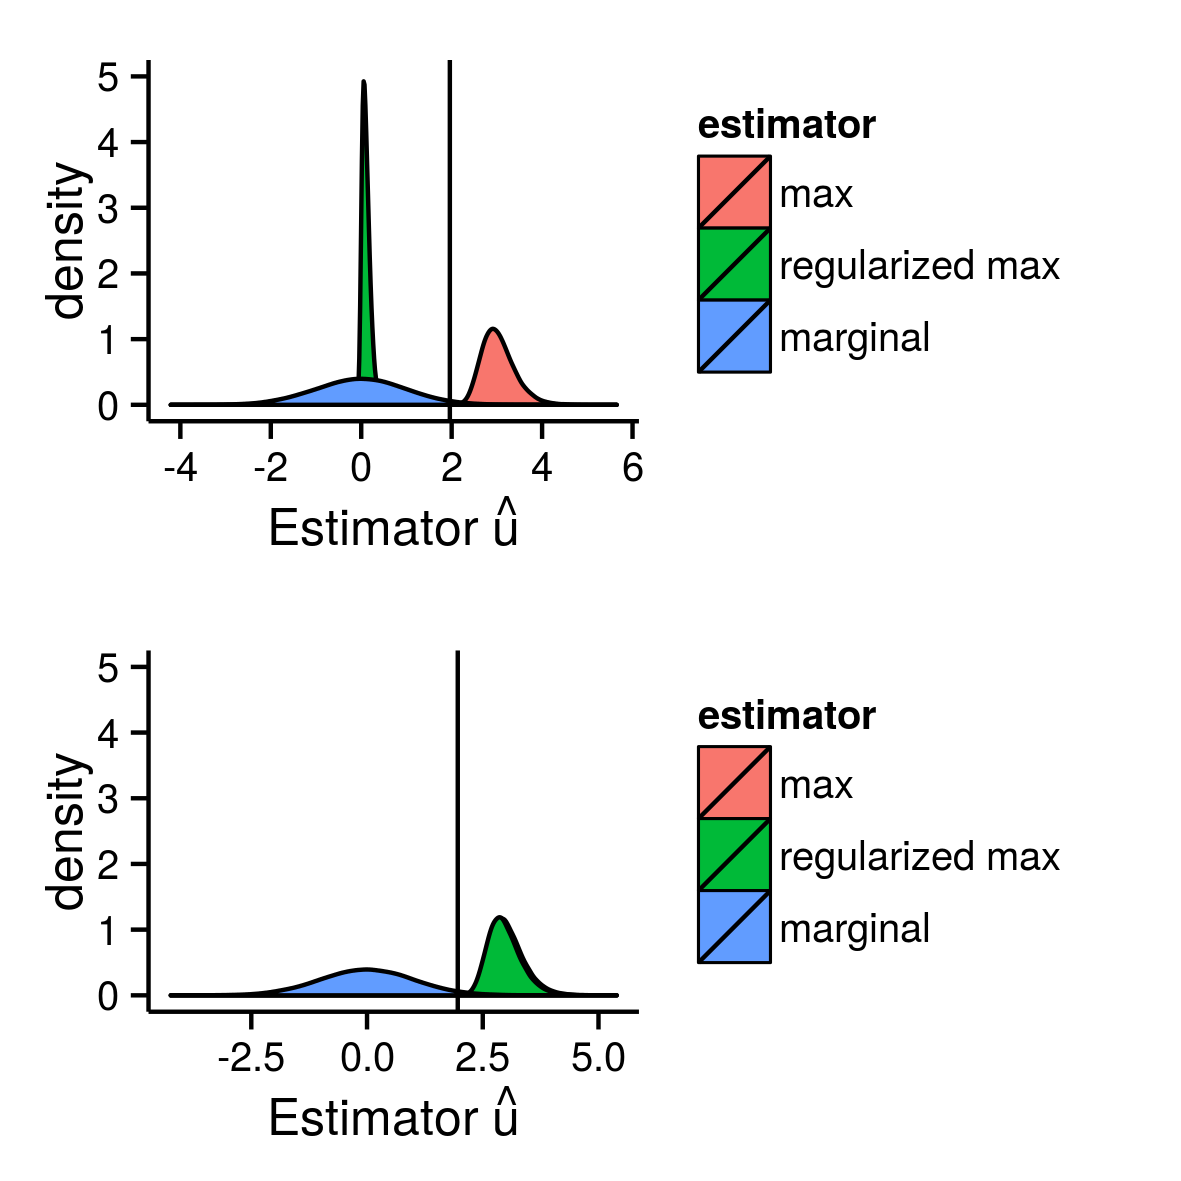
\includegraphics[width=10cm]{fig}
\caption{The marginal distribution of one element $\hat{U}_i|u^*$ of a classical signal estimator $\hat{U}|u^*$ in blue, the distribution of the maximum of that classical estimator $\hat{U}_{max}|u^*$ in red, and the distribution of the maximum hierarchical Bayesian posterior $U_{max}|v,u^*$ in green (see text for details of notation and simulation). The vertical bar illustrates the (uncorrected) test threshold $h$, that would only be correct if our signal had exactly one element, i.e. $|I|=1$. Instead we assume $|I|=100$. Under the family null $u_i=0,\forall i$ (upper plot), the maximum signal estimator in a classical, non-hierarchical model demonstrates extreme over-estimating, deviating far from the true setting of zero. Classically, this requires increasing $h$ to correct for multiple tests. In contrast, the posterior signal maximum of our hierarchical Bayesian model automatically shrinks to beneath $h$. Critically, this restriction on posterior inference is adaptive to the data. It is automatically lifted when the underlying signal is not null (lower plot), i.e. when latent target signal $u$ is more complex and $u_i \neq 0$ but in fact varies randomly over $i \in I$. In the lower panel it was sampled from a non-null signal distribution on $U$ with $\psi_U=(\mu_0,\tau_0)=(0,1/10)$. This is reminiscent of adaptive testing, in which the test threshold - rather than estimator - changes according to inferred signal variation. }
\label{fig:regularized maxima}
\end{figure}


\subsection{Details of Simulation}

Using real data from X, we compared frequentist and Bayesian inference on a parameter that we knew to be $0$, by ground truth, over the whole brain.

1) We first estimated the GLM parameter associated with a single random regressor (independent, standard Gaussian realizations), using both frequentist SPM and Bayesian PPM schemes. The frequentist estimation scheme provides us with uncorrected $h_u$ and the corrected $h_c$ (from the standard approximate SPMM survival function at high $h$). We used Monte-Carlo simulation to estimate the corresponding PPMM survival function. We simply sampled from the joint posterior PPM and choose the maxima (this gives a PPM maxima distribution, comparable to the SPM maxima distribution given by RFT etc). Specifically, we sampled from the PPM maxima distribution by first drawing $1000$ samples from the N-dimensional joint PPM, then extracting the observed maxima over the entire brain. The proportion of these realized maxima which exceed $h$ is called a Monte-Carlo estimate of $BEP_h$. 

2) We used permutation Monte-Carlo to assess the SPM maxima distribution non-parametrically. This has the advantage of giving us (an estimate of) the entire SPM maxima distribution (where the RFT approximation is only valid for high thresholds). We can then see unambiguously that SPM maxima dominate PPM maxima.

The data can be found at:

http://www.fil.ion.ucl.ac.uk/spm/data/face_rfx/

http://www.fil.ion.ucl.ac.uk/spm/data/face_rfx/face_rfx_spm12_batch.m

Henson, R.N.A, Shallice, T., Gorno-Tempini, M.-L. & Dolan, R.J (2002). Face repetition effects in implicit and explicit memory tests as measured by fMRI. Cerebral Cortex, 12, 178-186.

\section{Hierarchical Bayesian stochastic process models}

Moving beyond the specific examples above, we now consider hierarchical modeling more generally. ``Hierarchical'' modeling is based on the fact that the joint distribution of a set of random variables decomposes into a series of smaller, conditional models. All hierarchical models - spatial, temporal, neither or both - are formulated in three levels (possibly with sub-levels).

Parameter model: [noise-parameters $\psi_V$ and signal-parameters $\psi_U$]

Hidden signal model: [signal $U$ given signal-parameters $\psi_U$]

Observed data model: [outcome $V$ given signal and noise-parameters $\psi_V$].

This hierarchy may be written 
\begin{equation} \label{eq1}
\begin{split}
\psi = (\psi_U , \psi_V) & | S\\
U & | \psi_U, S\\
V & |U, \psi_V, S\\
\end{split}
\end{equation}

This notation can be interpreted generally, so that $\psi_U$ ($\psi_V$) are the signal (noise) parameters of any arbitrary hierarchical model, and not just the inverse-precision parameters of our simple linear-Gaussian example model above. $S$ denotes the (often implicit) model-specific, parametric and conditional independence constraints within and across levels. Here $U$ is  a general stochastic process\footnote{Recall that a \textit{random variable} $U_i(\omega)$ is any measurable, real-valued function of the outcome $\omega \in \Omega$ of a random experiment: the random $\omega$ means $U_i(\omega)$ is also random. Each experiment generates a specific outcome $\omega$ and therefore a specific real number $u_i = U_i(\omega)$. A \textit{stochastic process} is simply a set of random variables $U(\omega) \equiv \{U_i(\omega): i \in I\}$, indexed by some index set $I$. Depending on the model, this index set may be discrete or continuous, countable or uncountable. Here an outcome $\omega$ implies a whole set of real numbers, $u \equiv \{ u_i : i \in I \} \equiv \{U_i(\omega): i \in I\}$. For clarity we omit the argument $\omega$ throughout.}.

We have emphasized that knowledge of the generating process or distribution on $U$ constrains which samples are probable and credible: infering and applying this constraint therefore limits over-fitting/testing under the family null. To understand distributional constraints on a general stochastic process $U$ it helps to ask whether two arbitrary process subsets $U_A \equiv \{U_i: i \in A \}$ and $U_B \equiv \{U_i: i \in B \}$, indexed by possibly overlapping index subsets $A$ and $B$, are statistically and/or parametrically dependent\footnote{It also helps to ask whether the process index-set is a finite subset of natural numbers, a graph-valued index set, a (uncountably infinite) subset of real euclidean space or some non-euclidean topologies.}. Statistical dependence implies the restriction that $U_A$ and $U_B$ are not free to vary independently, $p(u_A,u_B|\psi_U) \neq p(u_A|\psi_U)p(u_B|\psi_U)$. Parametric dependence means they are not free to differ arbitrarily in \textit{marginal} distribution, but must share common signal parameters, i.e. $p(u_A|\psi_U), p(u_B|\psi_U)$. Just as in our simple example, inference on these general constraints can help adaptively control posterior error variation. 

We have said that $U$ may be constrained by qualitative (in)dependence constraints, not just quantitative hyper-parameters. Permissible statistical dependence may be represented by the edges between nodes of a graph (all random variables in the hierarchical model get a node): a missing edge between two subsets of the process implies a conditional independence. For example, $U_A$ and $U_B$ may be conditionally independent, conditional on (hyper)parameters $\psi_U$ alone (e.g. global shrinkage priors and our simple example), or independent given parameters $\psi_U$ and some other set of signal $U_N$ (e.g. the neighbourhood $N$ separates them, as assumed in Markov random field spatial prior) or independent asymptotically  as $A$ and $B$ become separated by increasing, continuous distance (Gaussian diffusion priors). 

Parametric dependence - e.g. identical parameters - refers to relationships between parameters of the marginal distributions on $U_A$ and $U_B$. Such dependence arises when the joint distribution over finite subsets of the signal process remain identical under some transformations of the index set $I$. For example, ``exchangeability'', ``stationarity'' or ``isotropy'' describe invariance of all finite subsets of the process to permutation, translation or rotation, respectively. (These invariants of the process imply that process subsets share \textit{all} parameters, because two finite subsets share identical joint marginal distributions! For this reason we refer to ``parametric dependence'').

Another very general restriction on a process is the assumption that it follows some known parametric form. The most common spatial priors in neuroimaging are a convolution of Gaussian processes: Either conditionally white processes (global priors in PPM), Markov-conditionally white (local shrinkage ``spatial'' priors) or asymptotically white priors (badly named ``Gaussian process'' priors, parametrized by some kernel $K$). Relaxing these parametric restrictions leads to non-parametric stochastic processes (e.g. spatial Dirichlet process) which go beyond our current scope. 

The qualitative issues which we have discussed dictate whether, given family null data $V^*$, $U_{max}|v^*$, and conditional Bayesian FWER, can be controlled by hierarchical inference. Precisely quantifying such control is a larger job which we only begin in this work\footnote{The most extreme value - and the topological complexity - of a process increases with the size (or Lesbegue measure) of index set $|I|$, the point-wise variance at each $i \in I$ and the independence across $i\in I$. Shannon's information entropy also increases with size, marginal variance and joint independence but is more general, and applies to nominal random variables, such as class labels, for which extrema are meaningless. Because entropy increases with the dimension $|I|$ it is used to regularize the dimensionality of probabilistic PCA/ICA decompositions. Relative entropy - or KL divergence - of prior and posterior process offer a general way to understand Bayesian control of over-estimating. For example the celebrated ``model evidence'' or ``marginal likelihood'' of our signal parameter $\psi_U$ can be written as $p(v|\psi_U) = exp(E_{u | v, \psi_U}ln p(v| u, \psi_U) - KL(p(u|v,\psi_U) || p(u|\psi_U)))$. This says that the posterior deviations from the prior distribution $KL(p(u|v,\psi_U) || p(u|\psi_U))$ incur an exponential penalty (again KL is relative entropy).}.

\section{Spatio-temporal neuroimaging}

We now illustrate how these concepts relate to neuroimaging. Functional imaging measurements $V_s_t$ are typically indexed by space and time, $V = \{V_{st} :s \in S, t \in T\}$. The ``continuous field'' perspective on such data recognizes that the sets of time $T$ and space $S$ are continuous: technology alone limits our measurements to a finite subset of points. In contrast, the ``discrete field'' perspective restricts itself from the outset to considering \textit{aggregates} over small continuous regions of space and/or time, e.g. indexed by discrete scan and voxel number.

Consider the general model $\{V_{st} : V_{st} = f(x_{st},u_{st}, e_{st}), s \in S, t \in T\}$ where the observed data is related to three other quantities - a known vector of predictors at each space-time $\{x_{st}\}$, an unobserved target vector $\{u_{st} \}$, and unobserved noise $\{e_{st}\}$ which corrupts each measurement (for notational clarity, we omit the condition $s \in S, t \in T$ on each of these sets). Note that $\{u_{st}\}$ is a large set of unknowns, e.g. number of scan-times x number of spatial voxels x dimensionality $C$ of our vector $u_{st}$. Naive attempts to fit our model to data (or test) will suffer from a serious ``over-fitting'', ``multiple estimation'' or ``multiple testing'' problem, arising from the aggregation of small estimation errors over a large signal.

A conventional solution would be to assume some equality constraints on the spatio-temporal expression of signal $u$. For example, neuroimaging analyses typically assume the unknown vector $u_{st}=u_s$ and $x_{st}=x_t$. Thus $u_s$ at each spatial position $s$ is a time-invariant ``fixed effect'' with respect to time, and  the predictor $x_t$ is space-invariant. These help limit temporal over-fitting at any point in space\footnote{A typical analysis additionally assumes linearity in the unknowns $\{u_s,e_{st}\}$, i.e.  $V_{st}= f(x_{st},u_{s}, e_{st}) = x_{t}^Tu_{s} + e_{st} = \sum_{c \in C} x_{tc}u_{sc} + e_{st}$, conveniently permitting us to write the observed data in matrix notation as $V=XU+E$. Here the visible data $V_{st}$ is arranged into a $N \times V$ matrix (number of measured time-points $\times$ number of measured space points), $X$ is a space-invariant experimental design matrix (N $\times$ number predictors $C$), unobservable parameters $U$ form a $C \times V$  matrix, and $E$ is a $N \times V$ matrix of stochastic errors.}. This reduces the inference problem to $C \times V$, which nonetheless remains huge.  

I change indices from st to ij!

Conventional ``region-of-interest'' analysis attempts to rescue this situation through another appeal to equality constraints, namely $u_{s}=u_{s'}=u$ for all $s \neq s'$, i.e. unknown parameters are invariant over some spatial region. This reduces estimated signal down to one $C$ dimensional vector. To summarize, the region-of-interest constraint $u_{st}=u_{s't'}=u$ restricts how much independent signal there is to over-fit down to just the $C$ components of $u$. This comes at the expense of introducing under-fitting bias whenever the signal $u$ is not really time or space invariant. How can we assess whether such constraints are appropriate? In principle, one could use some ``omnibus'' test of the family null hypothesis, e.g. $u_i=u_j$ for all $i,j$. This is akin to the familiar conventional F-test, which is parametrized by the number of constraints imposed (possibly adjusted for non-sphericity). Generally such testing requires the conditional frequency distribution of a scalar model comparison index, example maximum likelihood ratio, given the null setting/model. In reality, practitioners seldom perform this test. This amounts to infinitely precise priors on the constraint. In principle this constraint can be rejected by model comparison with either a more general conventional or hierarchical alternative. Don't test prior on the family null. 

Moving beyond region-of-interest analyses, in general there are untested equality constraints implicit in all conventional forms of pre-specified spatial smoothing. These go from the simple identity $u_i = u_j$ assumption above to assumptions about stationarity such as $u_i=u_{i-k}$ or isotropy such as $u_i-u_j=f(|i-j|)$. The hierachical approach replaces these with \textit{statistical} constraints of exchangeability, stationarity or isotropy, see "Hierarchical Bayesian stochastic process models". In practice this means that fixed equality constraints such as $u_i=u_j$ or equivalently $u_i-u_j=0$, are replaced with random equality constraint $p(u_i -u_j}|\psi_U) \approx 0 $, sometimes expressed in terms of a discrete slope between neighbours $p((u_i -u_j)/\delta|\psi_U) \approx 0 $ (or continuous derivative), the covariance $cov(u_i,u_j|\psi_U)$, etc. Importantly, these restrictions are not pre-specified, can be imposed - or relaxed - by different, inferable settings of $\psi_U$. \\

\noindent\fbox{%
\parbox{\textwidth}{%
\textit{Future research:}
Use simulation under other existing spatial imaging models, to confirm that they incidentally control FWER.

Use global shrinkage with a spatial structural/neuromodulatory predictor. This would provide a way to functionally validate structural models, and to test whether spatial distribution of neuromodulator predicts fMRI. 

Bayesian model selection over space, that incidentally controls FWER.

Validate connections between hierarchical control and FDR.

Hierarchical regularization of noisy single trial ERP.

Nested PPMs: scale-space PPMS! Easy!

}%
}

\section{Conclusion} 

Power boost by weakening the critereon - FDR over FWER - or stengthening the dependence assumptions - positive correlation BH versus any dependence BY - or my adjusting only for the number of null tests - adaptive methods\footnote{if we only knew the number of true null hypotheses, or the sparcity -  we could adjust for it instead of m, giving us larger cut-off values. It is fairly easy to estimate m0 given many tests, e.g. Storey method)}.

HMs imply a correlation structure between tests?

The idea of moderation comes from Stein's paradox [1].  In its simplest form it states that when you are estimating 4 or more population means, the best estimator is not the 4 or more sample means, but a weighted average of the sample means and the "mean of the means".  One way to find an appropriate weighting is to assume that the population means themselves come from a population (which is a Bayesian idea).  This population is then the prior, and the best estimator of each population mean is the Bayes predictor, which is a weighted average of the prior mean and the sample mean.  LIMMA uses an Empirical Bayes method which estimates the prior from the set of all feature(since we have 2000 of them - one for each gene).


Tension: want some assumptions must be true in order to ``falsify'' others. For example, the truth of the Gaussian assumption permits us to use Gaussian theory to reject a hypothesis test of group differences in the mean.

Kolmogorov smirnoff: want data to be consistent with a null.


Reproducibility of the arg-max $u_{max}$, and ranked lists more generally.

Explain and subtract unobserved differences/distance/heterogeneity(variability for frequentists).  For example, the relationship shown in Figure 1 explains approximately $34\%$ of variability in individual gene expression variances. 

Constraints intended to only reduce variance can risk bias if they are misspecified.
Can't draw on law of large numbers (of replicate samples), so assume ``pseudo''-samples, in the guise of samples from exchangeable experiments or conditions.
Incorporate/Combine all sources of information about unknowns. Jointly co-informative sets, e.g. exchangeable sets.

An additional source of information not commonly utilized in the statistical analysis of microarray data is the well documented dependence of gene variances on overall expression level of corresponding genes. 

Strong assumptions.
Quote: “Resampling” is a general term that encompasses bootstrap, permutation, and parametric simulation-based analyses; “resampling-based multiple testing” refers to the use of such methods in multiple testing applications. Resampling methods have become popular for “-omics” because they (a) require fewer assumptions (e.g. normality) about the data-generating process, thereby yielding procedures that are more robust, (b) utilize data-based distributional characteristics, e.g. discreteness and correlation structure, to make tests more powerful, and (c) scale up reasonably well to high-dimensional settings, particularly with modern computing.
dispensing with all assumptions about the data-generating mechanism... We won't even assume that the data necessarily arise from a random process. This framework is similar to the simple falsification approach to non-multiplicity corrected hypothesis testing. For example, to test H0 : μ = 0 using a t-test, the i.i.d. N(0; σ2) assumptions all form the null hypothesis. No assumption is needed otherwise if you only want to control the type I error rate. Rejection of H0 in this setting does not necessarily imply μ ≠ 0; rather, it implies rejection of independence, identical distributions, normality, or μ = 0 (or, by the central limit theorem, in large samples it approximately implies rejection of independence, identical distributions, or μ = 0). The conclusion μ ≠ 0 follows only if one is willing to accept all the other assumptions. The “other assumptions” are what we avoid altogether: everything will be embedded within the null hypotheses. We do this by using permutation tests, which allows for elegant theory, but a similar theory might be developed using other tests. This approach of embedding all assumptions into the null hypothesis may not be ideal, from a research standpoint, because rejection of the null hypothesis may give the researcher little information as to why the hypothesis was rejected. Nevertheless, a major contribution of this paper is the development of this point of view in the multiple testing arena. We show, despite the very minimal setup, that a reasonably powerful and flexible class of multiple testing procedures is obtained.
In fairness, the elements of the “framework” are restrictive; for example, if the researcher is only interested in location shift effects, then he or she is not interested in permutation tests. However, as stated above, the elements of the “framework” are somewhat different from the probabilistic assumptions that are usually made about data-generating processes. ...Hi is tested using a real-valued test statistic that is a function only of the data in
variable i: (JC: not so for us!)
Furthermore, much in the spirit of multiple testing adjustment mentioned in Section 3.1.1, the bootstrap provides a powerful way for simultaneous inference where the dependence structure of √n(ˆbj − βj0)/ Ωj,j across j is automatically taken into account.


With these elements, closed testing can be performed to control the FWE, entirely free of probabilistic assumptions about the data-generating process, other than what is embedded in the null hypotheses. .
   
We have seen a bewildering variety of multiple testing procedures. How should we choose which to use? There are no simple answers here, but each procedure can be judged according to a number of criteria. Interpretation: does the procedure answer a question that is rele- vant to the analysis? Type of control: weak, exact or strong? Validity: are the assumptions under which the procedure is valid definitely or plausibly true, or is their truth unclear, or are they most probably not true? And finally, computability: are the procedure’s calcula- tions straightforward to perform accurately, or is there substantial numerical or simulation. 

It will take a while before we accumulate enough experience to know which approach leads to truer biological conclusions on a large scale, that is, which in truth better balances false positives and false negatives in practice. The FWER-based maxT procedure successfully identified the 8 differentially expressed genes in the Apo AI dataset which have been biologi- cally verified, though the identical distribution assumption is highly doubtful, see below. For the Golub leukemia dataset, maxT gave a smaller number of differentially expressed genes than the FDR-based procedures, but no large scale validation has been done to determine the truth there. It seems possible that when just a few genes are expected to be differen- tially expressed, as with the Apo AI dataset, it might be a good idea to use FWER-based procedures, while when many genes are expected to be differentially expressed, as with the leukemia dataset, it might be better to use FDR or pFDR-based procedures.  
The strength of maxT and minP is that they are exploiting the dependence in the test statistics in order to improve power. By contrast, the Sˇida ́k, BH, Storey and ST procedures are motivated by independence (and perhaps identical distribution) assumptions on the test statistics. They try to extend results valid under independence to more general situations by imposing special conditions: the Sˇida ́k inequality for the Sˇida ́k procedure, positive re- gression dependency for BH, and ergodic conditions for the Storey procedure. For a start, it is difficult to see how we can be sure that these conditions apply with microarray data. 

In addition to the multiplicity issue mentioned before, another potential problem is that if the data are not normally distributed, applying a t-test can be invalid when the sam- ple size is small1. However, this problem is not the focus of the current primer, in which the data in our example are assumed to be nor- mally distributed.
genes. The validity of model assumptions, such as those on the hierarchical structure and the distributions at the top and bottom levels, is crucial for the successful application of hierarchical models. When the assumptions hold true, the model brings additional power. Otherwise, the model may not use the infor- mation optimally, or may introduce bias that leads to misleading results. Therefore, it is always wise to check the model assumptions by exploring characteristics of the raw data and testing the analysis results using inde- pendent information or cross-validation2.

However, the Bayesian hierarchical model approach can suffer from the ‘over-correction’ problem and produce false negatives. In addition, it assumes a common prior for every gene, which will limit the effectiveness of the approach for genes with dramatically different behaviors. In contrast, IPBT assumes gene-specific, informative priors. With the rapid proliferation of high-throughput genomics big data, deriving these informative priors is no longer an issue.

Meta-analysis is a powerful tool for combining multiple studies of a related hypothesis and has been applied to microarray data (Conlon et al., 2007; Tseng et al., 2012). Our approach is different from meta-analysis because historical data used in IPBT may come from experiments with a different hypothesis, and the historical data is used indirectly in the form of informative priors in Bayesian inference.

discriminate random vs reproducible association.
The models are useful in a broad spectrum of large-p problems where their is low information per locus, low small sample size being a special case. For example, predicting transcription factor binding sites in DNA sequences can be viewed as a problem that probabilistically assigns a 0–1 label to each locus by matching the sequence to a motif model as opposed to a background model.

This weighted average technique to estimate the variance is called variance stabilization. HM inference ``indepenent'' or ``robust'' to unexplained observation error. It is widely used in analyses of gene expression microarrays4,8 and chromatin immunoprecipitation on til- ing microarrays (ChIP-chip)7 to detect dif- ferentially expressed genes and protein-DNA binding sites, respectively. Naturally, real microarray experiments are more complicated and contain more sources of variation than our example; thus, they can benefit from more sophisticated hierarchical models that capture those types of variation.

Small sample sizes result in imprecise estimates if each gene $u_i$ is considered independently.
 
Maximum $\max_{i \in I}U_i$ is a non-linear function on a process. Contrast with other functions on $U$, say $\sum_{i \in I} U_i$, which may be linear.

Our confidence in a conventional interval comes from the fact that the inference method we used works on average over repeat sampling from the DGP. Confidence in a Bayesian interval summarizes uncertain belief about the unknown true value in our specific sample.

Which assumptions underly precision/identifiablity gains: identical parameter vs identical distribution. Limma is an empirical Bayesian method, which uses a hierarchical similarity across genes, reduces component to component differences, e.g. the norm (Smyth, 2004). Ideal information source (to increase precision) has identical/similar values (then shrinkage is strong). Instead of borrowing information from different genes measured in the same experiment, our proposed approach borrows information from the measurements of the same gene in different ex- periments conducted in the past, using the same technology, same type of chip, on the same type of cells (or similar). The main dif- ference between IPBT and the hierarchical model in (2)–(4) is that here hyper parameters ( i;x2i ) for the variance r2i s are gene-specific.
Hierarchical stabilization or shrinkage - borrowing strength - b

Bias and variance in estimators, e.g. causal or non-causal parameters of population. 
For causal inference: bias - simpson confounding, berkson selection - is bad.
Unbiasedness - or at least known shrinkage bias - is important in casual inference. 
Pearl has alot to say about bias in estimation of population causal parameters and individual causal states. He defines it clearly, and enumerates.
Not much on variance.
Bias wrt the true population parameter. Bias with respect to a causal population \textit{parameter}. Bias in individual level causal \textit{inference} (Pearl). 
Bias: Ecological/Simpson's bias is an underfitting bias. Selection bias is not. diagnose by DAG, prevent by randomization. Measurement bias. Big data problems (don't average out in big data).
Variance: Random sampling error of estimator = random deviation of estimator due to random sampling from population.
Frequentist bias-variance tradeoff: bias useful (especially if we \textit{know} the bias, e.g. shrinkage bias given by $\hat{\psi}_U$).

Avoid biased population estimators by random selection, random intervention (assignment of units to treatments).
Sampling selection bias (berksons non-random sample selection) versus simpsons modeling (underfitting) bias.
Non-random intervention (confounding such as paradox). Experiment. 
Blocked randomized replicated experiment for bias-variance reduction: Block for variance-reduction, then randomize within block for bias-reduction. This randomization increases variance - randomization variation cf sampling variation just named after the source - in causal estimators. So use replication.

Re-randomization/pemutation test (units randomized to treatments, re-randomize), Re-sampling estimator. 

FWER ignores different costs of error.
Incorrect/correct decisions have different costs for different stakeholds: a game. 

Many treatments of multiple testing focus on $p-values$. In general a decision on one $p-value$ is not $seperable$ but can depend on all $p-values$: this pays off when test statistics, and therefore $p-values$ are dependent.

FDR control via BH rests on ordering the p-values. Under the homogenous variance assumption in our simple example, the only thing that differs between $i \in I$ are the components of $u$ itself. So an ordering of p-values reduces to ordering on estimated effect sizes $\hat{U}$: BH accepts $\hat{U}_{max}$ if its p-value is beneath $\alpha/m$.

Often it is unsafe to assume a parametric form for the population process, as we have throughout.


Multilevel models support multilevel generalization: in a parametric, nested design for example this means generalizing to new data from a subject $\psi_V$ versus to new subjects $\psi_U$. The parameters $\psi_U,\psi_V$ respectively govern generatization to new indices $i',j'$ in $V_{i',j'}$ respectively (of course generalization may be local to one dimension of the index set).

Our work develops on Gelman et al. (2012). The FWER of $0.05$ or even $0.001$ is arguably far too low.

Conventional control of \textit{test} error incidentally reduces \textit{estimation} error because complete data/parameter pooling is the default, unless the null can be rejected. We have emphasized that, conversely, hierarchical control of estimation error incidentally reduces hierachical test error. Thus, using either quantitive estimation or qualitative testing, the result is comparable: one correction is enough. In our simple example, the hierarchical control parameter $\psi_U$ mimicks the conventional test control parameter $h_{\alpha}$. ($h_{alpha}$ is a parameter of the decision rule, $\psi_U$ is a parameter of the data-generating process: that they both control over-fitting means decision rules can but need not be explicitly be designed to reduce aggregate error).  Both shrink or nullify model complexity under the family null hypothesis, implementing an Occam's razor. 

To relate these two schools we considered the multiplicity problem. We emphasized that scale of this problem increases with signal dimensionality in ``large-$u$'' problems, incurring a severe ``multiple test problem''. This error may be seen in the distribution of maximum estimator under the family null, for which $\mathbb{P}(\hat{U}_{max}^* > h) \leq \mathbb{P}(\hat{U}_{max}^* > h)$, for any $I \subseteq I'$ and some null $u^*$. Thus, the probability that a big error ($>h$) arises somewhere in $\hat{U}$ increases with the size/volume of the signal vector (all else constant). We showed that in hierarchical Bayesian analysis conditional on family null data this condition is reversed i.e. $\mathbb{P}(\hat{U}_{max}^* > h|v^*) \geq \mathbb{P}(\hat{U}_{max}^* > h|v,u^*)$. Thus multiplicity can be a blessing, not a curse for hierarchical models. The maxima provides one way to illustrate how hierarchical inference can automatically solve the over-estimating/testing problem.

Weak control of FWER? When the family null is false.

The general generating process for $U$ gives information on the credible values of $u$. Conversely, the (noise-corrupt) $u$ gives information on the generating process $U$. 

We have shown here that both hierarchical and non-hierarchical procedures control false-positive error rate. This does not make them equivalent. Control of false-negative error is vastly worse in conventional procedures. The problem with conventional procedures in principle is underfitting not overfitting. Conventional procedures take great care to control false-positive error, strictly penalizing complex models with too many unconstrained parameters. They do this by assuming a simple null model by default, unless the null can be rejected by a test. In large-scale conventional inference, post-hoc test corrections which weakly control FWER assume the family null by default. This framing completely neglects false \textit{negatives} which arise if the family null is false. This means underfitting, or oversmoothing true effects. Hierarchical procedures avoid this trap by infering the plausibility of the family null first. Shrinkage is relaxed when the family null is implausible: this reduces false negative errors. Otherwise, shrinkage penalizes false-positives.


"The classical approach to the multiple testing problem relies on constructing procedures maximizing the power while controlling FWER"

 
There are different ways to quantify aggregate inferential error, for example, the family-wise error over tests, the mean squared error over estimators and the maxima error over estimators. Conventional procedures prioritize the first, hierarchical procedures the second (James-Stein). We propose the third metric, the estimator maxima, bridges these approaches. In particular, the maxima distribution shows why conventional test correction is necessary under the family null, and why hierarchical test correction is not. Non-uniform priors are analogous to ridge regression, whose out-of-sample predictive performance exceeds least squares because it penalizes the sum of squared estimators.

We have shown that hierarchical Bayesian inference weakly controls frequentist FWER at uncorrected test thresholds, both conditionally and marginally. We do not recommend uncorrected test thresholds as standard practice when reporting Bayesian posterior inferences.

Conventional and Hierarchical methods differ in their treatment of unobserved heterogeneity across members of some index-set $I$. The conventional approach can only reject equality constraints, while hierarchical approach learns the complete latent sampling process.

Non-hierarchical inference, both Bayesian and frequentist, uses fixed constraints to limit overfitting: a fixed Bayesian prior or a fixed null hypothesis. To avoid overfitting large models, these constraints increase with the problem dimensionality or "multiple comparisons" (DCM prior precision depends on number of params, same for MCP). Hierarchical procedures - Bayesian or frequentist shrinkage or FDR - do not use fix constraints, blindly increasing constraints with the problem dimensionality. Instead constraints are derived from the data itself. This means overfitting is penalized more when the family null is plausible \texti{a postiori} (not when it is simply higher dimensional). In our simple example, hierarchical learning means infering $\psi_U \approx \infty$ from data. 

Conversely, when the family null is implausible, false-positive error control is relaxed and false-negative error is reduced. Herer inference on component $u_i$ is freed from hierarchical constraint. For hierarchical Bayesians the family null is a (degenerate) latent generating process, in other words a point mass on the $0$ vector: the choice of whether to police false-positive versus false-negative test error - equivalently over-fitting versus under-fitting error - is made automatically, by infering the family null plausibility. For non-hierarchical procedures, the family null false-positive error is \textit{assumed}, even if it is not plausible given the data. These procedures therefore blindly penalize false positives, parameter overfitting or model over-complexity, even when false-negatives, underfitting or model over-simplicity are the real problem.

Pedogogy: 
1. show target realization
2. show likelihoods (with dispersion, each only centered on target in expectation)
3. now remove the target realizations and show generating process instead, explain that if you had to choose amoung likely arguments of the (dispersed) likelihood function, you'd probably favour the shrunk side. This is bayesian analysis.
4. now hide the generating process, can it be learned by hierarchical learning (MLII, full Bayesian or whatever).

decision theory: control! i.e. min EL(s,a)
causal theory: control!

\section{Appendix 1: A simple example}
Given $\psi_U,\psi_V$, it can be shown by Bayes theorem that uncertain posterior inference on the latent sample realization $u_i$, denoted $U_i|v,\psi_U,\psi_V$, is also Gaussian, with precision parameter equal to $\psi_U+n\psi_V$ and mean parameter equal to $\frac{n\psi_V \hat{u}_i}{\psi_U+n\psi_V}$, where $\hat{u}_i = \frac{1}{J_i}\sum_{j=1}^J v_{i,j}$ is the observed sample mean. These equations show that a large prior constraint - large $\psi_U$ - on the sampling process $U_i$ causes the posterior mean inference on realization $u_i$ to shrink towards zero and away from the observed sample mean $\hat{u}_i$. Posterior uncertainty about $u_i$, given by variance $1/\psi_U$, also shrinks to zero, effectively trapping all posterior mass close to zero. These facts are useful because the \textit{estimated} distributional constraint $\hat{\psi}_U$ should be large when the family null is true: plugging this estimate into the formulas for the posterior mean and precision above will naturally shrink all posterior components $U_i|v^*, \hat{\psi}_U, \hat{\psi_V}$ towards zero. It is by this mechanism that hierarchical methods suppress noise or counter over-fitting under the family null hypothesis. 



\section{Appendix 2: Different types of maxima}

We should clearly distinguish different maxima. Given a specific set of, typically unobserved, real numbers of interest $u \equiv \{u_i: i \in I \}$, $u_{max}$ is just the largest value in that set. Given a conventional noise-corrupt estimator of $\hat{U}(V)$ of $u$, $\hat{U}_{max}(V)$ is the distribution of the maximal estimate over repeated, noise-corrupt samples $V$ \textit{with $u$ fixed}. Assuming the family null means assuming $u_i=u_j=u_{max}=0$ for all $i,j \in I$. We denote ensuing family null samples $V^*$ and note $\hat{U}_{max}^* \equiv \hat{U}_{max}(V^*)$ can be used to quantify and weakly control FWER, see ``Classical maxima and conventional control''. 

Assume a general latent generating process $U|\psi_U \equiv \{U_i: i \in I \}|\psi_U$, then $U_{max}|\psi_U$ is the distribution of $u_{max}$ over repeat draws from the latent generating process. Bayesians might use this general sampling distribution as \textit{prior} belief about credible value of a specific unobserved $u_{max}$, i.e. the largest value in our $u$, see ``Bayesian and frequentist hierarchical inference''. One might call it the prior maxima distribution. Given Bayesian \textit{posterior} belief $U|v^*$ about our specific unobserved target $u$, $U_{max}|v^*$ is the credible posterior magnitude of our specific $u_{max}$. 

By Bayes theorem, $p(u_{max}|v) = p(v|u_{max})p(u_{max})/p(v)$, where $p(u_{max}) = \int_{\psi_U}p(u_{max}|\psi_U)$. The distribution of the prior maxima encodes maximum overfitting, i.e. over fitting that occurs without having data. $U_{max}|v^*$ encodes actual overfitting, conditional on family null data. ($U_{max}|v$, for non-null $v$, is not generally of interest.)

\section{Appendix on Bayesian versus frequentist inference}

Bayesians and frequentists differ in whether or not you can use probability to represent uncertainty about an unobserved constant, be it a fixed parameter or the unobserved realisation of random variable. Imagine a fair coin flipping process. The prospective relative frequency of heads is one half: this is the frequent notion of probability. If you believe a single, unobserved retrospective outcome was heads with probably one half, then you are Bayesian: a frequentist would say this is not random so has no probability distribution. 

Hierarchical predictions generalise to new latent realisations - via $\phi_U$ (and maybe all other data? c.f. Gaussian process) and new $x$.

Different components of the prior have different semantics. Prior to ignorance about what? What do we know about the unknown number, logical constraint $0<u<1$, sampling constraints, i.e. is it the realisation from a latent frequency distribution? For the latter, hierarchical, case prospective frequency - i.e. the population prior - dictates retrospective credibility of a sample. The outcome distribution is both the prediction for new data realisation, and subjective belief about an unobserved realization (which is no longer random, so frequentist cannot use probabilities). The prior predictive outcome distribution. The posterior predictive outcome distribution.


\section{note}

Frequentists attempt to interpret the estimates of the model, which is difficult except when the model is linear, has no inverse link function, and contains no interaction terms. Bayesians can avoid this difficulty simply by inspecting the posterior predictive distribution at different levels of the predictors.

\section{Strong versus weak control}

There are two popular hierarchical model classes for data with sparse and exchangeable signal (Carvalho horseshoe). The first models true sparsity, where $u_i=0$ for many of $i \in I$, by assuming that each $u_i$ is a mixture of a discrete point mass at $u_i=0$ and an absolutely continuous alternative. The second class models a weaker form of sparsity, where $u_i \approx 0$ for many $i \in I$, by giving the $u_i$ an absolutely continuous ``shrinkage'' prior, centered at zero. This latter includes the LASSO, relevance vector machine, horseshoe and standard ``global shrinkage'' PPM.

Numerical problems are common when estimating models from data with extremely sparce signal, such as under the FWN.

\section{Critique of global shrinkage PPM implementation}
The ReML estimates of the (hyper)parameters have precision linear in the number of voxels (Friston and Penny 2003).
Global shrinkage models observation error twice over. Once in Equ 4 of (Friston and Penny 2003) which is voxel-specific, once in Equ 7  of (Friston and Penny 2003) which ``can be treated as an estimate of the average [scale of observation error] over voxels''. These are combined into the approximation in Equ 10 of (Friston and Penny 2003). It is not stated whether Equ 10 shrinks or regularizes voxel-specific noise parameter estimation. 

The default arguments of a call to $spm_PEB.m$ from $spm_spm_Bayes.m$ for the purposes of second level global shrinkage PPM, permits negative error variance $h$.
PPM seems to overfit the observation noise parameters, there is at least one per voxel.
$spm_spm_Bayes.m$ then checks for them and ``corrects'' with $h = abs(h)$, which is dubious.
All ``random effect'' models make use of both fixed and random constraints. For example, a random intercept model typically assumes the error variance across component nested regressions is fixed, but regularizes the intercept. Model unequal variance parameters as random effects.


\section{Critique of global shrinkage PPM model}

Independent population prior on $\beta_0^i,\beta_1^i$ means voxel-specific intercept and slope are unrelated. If false, 

Traditional regression. Called between-voxel homoskedasticity in regression (different error variance) or homogeneity of variance assumption in ANOVA.


Heterogeneous noise and signal (i.e. both the scale of predictor coefficients and noise variance vary across voxels).

Three problems with PPM. Endogeneity from misspecification (residual dependence after modeling exchangeable voxel effects). Despite the model assumptions, the random noise errors are not conditionally independent across voxels, given random effects. Rather there are residual spatial correlations. Despite model assumptions, random effects may be correlated a priori. Nested model (subjects within voxels), but not nested data. The commonly tauted advantage is that submodels (1st level, nested regressions) with low-data benefit from sharing strength. In fMRI, data is balanced, with no voxel having more or less data. This means 

\noindent\fbox{%
\parbox{\textwidth}{%
\textit{Decision theory}

Optimal responses to an uncertain world rest on first defining our model of unknowns in the world - i.e. out-of-sample or fundamentally unobservable parameters/states - and then defining a model of the cost of taking each available action, given these unknowns. Under these assumptions, an optimal \textit{policy} is typically defined to be one which minimises the expected utility loss, a.k.a. the ``risk''. In learning/engineering tasks, for example, we often want to \textit{track} some unknown quantity, i.e. want decisions to match or fit an unknown quantity. The cost of mismatch is formalized by a ``decision-utility function'', e.g. expected squared prediction error loss (ESPEL) as below, a function which quantifies the (conditional) cost of each specific response given the fixed or random unknown quantity. (These two cases are called estimation and prediction respectively in statistics).

Thus a policy is a mapping from observable data to actions, known variously as a decision-rule, estimator, test, predictor, fitting-procedure/algorithm, statistic, etc. Frequentist statisticians try to devise good functions to identify and quantify hidden quantities of the world, assuming some model. These may be real-valued functions of the data (estimators), set-valued functions (confidence intervals or regions), binary-valued (``test'') functions, constructed to meet some desiderata. Statistically optimal policies invariably impose some constraints to adjust, penalize or correct for over-estimating, i.e. to reduce the probability of being ``far'' from the truth (estimators with small bias/variance) or ``false'' (tests small false-positive/negative).

Expected squared prediction error loss (ESPEL) exposes a general, famous trade-off between two sources of risk in any policy toward unknown parameters, states or out-of-sample predictions: ``statistical bias'' and ``statistical variance'', the first two central moments of the squared signal-prediction error. We ideally want zero statistical bias and variance. The trade-off says that, for any given risk, one can choose either but not both. ``Statistical bias'' captures the regular or predictable error over imagined replications of the data which arises due to a modeling restriction.  As explained in the text, this ``statistical bias'' relates intimately to ``inductive bias'' which helps extreme over-estimating by adaptive parameter shrinking. In contrast, statistical variance quantifies unpredictable, over-estimating error due to noise. The conventional school of inference typically takes a different view on this trade-off. Given the trade-off they prize unbiasedness and only then attempt to derive the minimum variance estimator. By pretending to circumvent inductive bias in inference they forgo the full power of hierarchical control of over-estimating.

``Analytic'' risk minimisation above differs from the ``Empirical risk minimization'' (in supervised learning models). This philosophy here is to approximate true risk by ``empirical risk'', i.e. the average loss function over some training set. The validity of this approach rests on correctly understanding the statistical properties of these cross-validation estimators of the true risk. We do not expand on these here.

}
}



\section{Notes}

%   The purpose of this class is to:
%   (1) Fit LME models in standard form by ML or REML.-
%   (3) Compute the estimate betaHat of fixed (effect) beta.-
%   (5) Compute the estimate sigmaHat of fixed sigma.-
%   (6) Compute the BLUP prediction bHat of b.-
%   (7) Estimate covariance of betaHat.-
%   (8) Perform hypothesis tests on beta.-
%   (9) CIs for contrasts of beta. -
%  (10) Compute covariance of [betaHat - beta;bHat - b].-
%  (11) Peform hypothesis tests on [beta;b]. -
%  (12) CIs for contrasts of [beta;b]. -
%  (13) Estimate covariance of [thetaHat;log(sigmaHat)].-
%  (14) Estimate covariance of [etaHat;log(sigmaHat)] where etaHat is the
%       Natural parameter vector for [thetaHat;log(sigmaHat)]. - 
%  (15) Compute confidence intervals on the canonical parameter vector
%       [heta;log(sigma)]. - 
%  (16) Compute conditional/marginal fitted values.-
%  (17) Compute conditional/marginal residuals of various types. -
%  (18) Generate random data from fitted model. -
%  (19) Make predictions on new data. -
%  (20) Compute the posterior covariance of random effects vector. - 


Testing or regularization of random and/or fixed parameters to minimizing noise in multivariate signal prediction/estimation. The non-hierarchical fixed-effects approach is to compare nested models, with versus without some functional restriction on signal. This comparison is possible for RFX models too (compare nested models with versus without some restriction on the variance component parameters). In addition, 

Identifiability problems whenever one random factor has zero variance (i.e. the null).

Optimal estimation and prediction entails stopping, shrinking, smoothing or filtering out noise variability. We perform an omnibus inference on the global null, by inferring the covariance component parameter which governs between-voxel random effects, e.g. in PMM with global-shrinkage prior. This substitutes a single comparison for multiple comparisons (akin to using a single F-statistic hypothesis test in linear fixed-effects models like ANOVA).

In PPM, voxels are indexed by the level of a categorical variable. PPM is a 2-level hierarchical model, with observations/subjects nested within voxels.

Despite PPM, subjects are crossed with - and not nested within - voxels. This model is not a ''hierarchical'' in Douglas Bates' terminology (but it is a multilevel).


A common example of wide linear models is when there are many exchangeable groups of observations, therefore parameters.

Regularized causal effect estimates. How to formulate and justify the regularization constraint.

Continuous or grouping (discrete, categorical) variable .

The design shapes the cost function/posterior over unknowns, i.e. the existence and curvature of a uniquely identifiable optima in the cost function over unknowns. Deterministic (linear) or statistical dependence (co-linear or correlated features) and the ratio of unknowns to observations. Co-linear or wide ($P>N$) designs imply there is no single unique optima, only a ''ridge'' of solutions. Correlated or sparsely observed features (e.g. $P/N \approx 1$) imply the unique optima is broad (large $\mathbb{V}(\hat{\beta})$). An inductive bias on the loss function - i.e. prior or ''regularization'' constraints on $P$ unknowns, such as some pre-specified unknowns are zero or equivalently omit variables so $N<P$, all unknowns should shrink towards zero (or some constant, c.f. Bridge regression), solutions must be orthogonal to non-principle components of the design (c.f. principle components regression), all unknowns are correlated $a$ $posteriori$, etc - ensures a well-posed optimization problem and reduces variance because there are more observations per parameter, but increases risk of under-fitting mis-specification bias. I.E. regularization bias reduces the number and breadth of optima to one precise optima, at cost of underfitting misspecification bias. With $N=P$ non-colinear features, the parameters fit the data perfectly, e.g. the data $are$ the parameters. As $P/N$ shrinks by inductive bias, $under-fitting$ $mis-specification$ bias increases but variance. Regularize an ill-posed and/or imprecise optimization problem. The omission inductive bias/constraint (unknown is prespecified to be zero) on the loss function only creates well-posed optimization if there is no remaining deterministic linear independence amoung included features. Pre-specified omission risks omitted feature bias in the right graph. Feature omission (zero weight/effect variable) constraints can induce bias, but so can feature inclusion (Pearl's selection bias). Omitted confounds is not the only source of bias. If loss is a function of unknown $causal$ parameters, can use Pearl's backdoor graphical criterion etc, to guide the variable/effect omission (pre-specified zeros) that do not incur bias, e.g. Simpson's causal paradox. For Pearl SEM-based ''identifiablity'' is not just due to the ratio of observations to unknowns or deterministic/statistical dependence among predictive features, but due to the open back-door paths with respect to the data generating process (omitted confounds, included colliders and/or cyclic causation). Also, increasing number of features/weights can reduce unexplained error variance, hence estimator variance (ceteris paribus, a.k.a. blocking).


Both frequentists/Bayesians aim to make predictions and to estimate parameters (where “parameters” are those aspects of a model that generalize to new data) Gelman's blog. JC: in my terms they are general or shared by all current and future indices. 

Gelman: lasso (by itself, and as an inspiration for Bayesian regularization) is a great idea.

identifiability and shrinkage via constraints (priors or penalties, which in turn can be learned by full Bayesian, empirical Bayesian or cross-validation methods)

regression coefficients getting out of control

I could go around smugly thinking that lasso was a trivial implementation of a prior distribution, coupled with a silly posterior-mode summary.

Discrete/continuous-smooth shrinkage of random parameters/states (alternatively, Lagrange constrained on regression). PCR and kernel PCR have a discrete shrinkage effect on the eigenvectors of. Contrast with Ridge regression.

Beware: correlated factors and/or failure to block on important factors both increase estimator variance. ''Extreme distance'': Hoeffding bounds, permutation p-values, parametric tests. Adaptive tests - e.g. Benjamini-Hochberg, and FWER analogies - adaptive estimation. Different thresholds + different interpretations for uncorrected, FDR, FWER.! Resolve endogeneity then resolve multiplicity. If assumptions are strong, uncertainty wrong, null is wrong (hence tests/p-values).

Rule of thumb: simple OLS ignoring/marginalizing over voxel-index (i.e. concatenate all voxel-specific data) is significant for a null effect, we have a problem!

Non-identifiable (e.g. infinite solutions because wide or co-linear design) or identified but noisy (non-orthogonal/correlated regressors).

This ”prior”, introduced before any access to the data, reflects our prior knowledge on $u$: general qualitative symmetries (e.g. exchangeability, which may modeled graphically) and quantitative parametric class assumptions such Gaussian (together with uncertainty about the ''hyper''-parameters). Posterior $distribution$ approximations can also rest on qualitative (e.g. mean-field) and quantitative (e.g. Gaussian) assumptions. Posterior $point$ approximation via MAP.

Lasso $\hat{u}(\lambda) = \underset{u}{argmin} \ \frac{1}{N} \sum_{i=1}^N (y_i - (u_0 + x_iu))^2 + \lambda \| u \|_1$

Ridge $\hat{u}(\lambda) = \underset{u}{argmin} \ \frac{1}{N} \sum_{i=1}^N (y_i - (u_0 + x_iu))^2 + \lambda \| u \|_2$

Because the log prior is a summation, the $u_1,...,u_I$ are mutually independent and identically distributed (white Laplacian or Gaussian process). We thus omit the subscript $i$ and study the prior distribution of $u$ (c.f. the bayesian bridge with R package $BayesBridge$). In spatial models, the $u_1,...,u_I$ are not independent, but spatially dependent. Parsimony of lasso: only a small subset of features  selected ⇒ increases the interpretability (especially conjugate with parcels). If n > m, i.e. more features than samples, Lasso will select at most m variables. More difficult to implement than Ridge Regression. 

Elasticnet (i.e. laplace * Gaussian prior, i.e. first and second bridge (or powered exponential) takes care of groups of correlated variables (and therefore effects) by shrinking together, but also selects them out. Selection or shrinkage?

R package $EBEN$ provides Empirical Bayesian Elastic Net (for wide, collinear and correlated designs).

''Hyperprior'' is a prior on the ''hyperparameters'', in Cressie this simplifies to ''prior on parameters'', all other effects are random.

R package $EBglmnet$ provides empirical Bayesian lasso and elastic net algorithms for variable selection and effect estimation (see $glmnet$ to learn hyperparameters by cross-validation instead). 

Almost nobody calls it “lasso.”  Lasso say (equivalently in terms of estimator) that they’re doing MAP with double-exponential (Laplace) priors.  The electrical engineers are all over L1 and call it “compressed sensing” for its motivating application in their world. Even the people fitting SVMs do it, and they rarely even talk about probability.

Ridge regression was invented - and named - as a solution to non-identifiability (ill-conditioned - e.g. ''wide'' or co-linear - designs). Its impact on $\mathbb{V}(\hat{\beta}^R)$ is what concerns us. \footnote{With multicollinearity, you get a ''ridge'' in the likelihood function (i.e. a trough in the Loss function such as RSS). Ridge regression ''fixes'' the ridge. The term ''ridge'' also relates to the main diagonal $\lambda I$ in $\hat{\beta}^R = (X^TX + \lambda I)^{-1}X^TY}$ which permits a solution to this inverse matrix. $\hat{\beta}^R$ is also the Bayesian MAP or posterior mean.}

standard errors for lasso and elastic net coefficients.

Figure: Binary nested model comparison by likelihood-ratio, or deviance difference $dd(l_1,l_2) = dd(l_1/l_2) = -2log(l_1/l_2)$ whose distribution in known ($1,2$ index nested constraints). If deviance $d(l_1,l_g) = -2log(l_1/l_g)$ then $dd(l_1,l_2) = d(l_1,l_g) - d(l_2, l_g)$. Fraction of deviance explained: as this approaches 1, we are perfectly overfitting.

Elasticnet provides identifiability via the L2 (i.e., “ridge”) component and shrinkage to 0 in point estimates via the L1 (i.e., “lasso”) component. Regarding identifiability, if you have two predictors x1 and x2 with perfect correlation, L2 regularization identifies a unique result, whereas with L1 regularization any interpolation between b * x1 and b * x2 (e.g. 0.3 * b + x1 + 0.7 * b * x2) has the same likelihood and the same L1 penalty (namely b). But the L2 penalty is lowest when the two coefficients are equal (lambda * b * x1 + lambda * b * x2). So you get identification.

Coefficients shrunk to exactly zero vastly reduces both the memory needed to store the model, and the time taken to compute a prediction. Whenever we set up a model with a finite number of variables we are already setting a lot of other parameters to zero! So don't critique lasso in this way. We all make binary distinctions all of the time (in/out of model, connected/not connected), so the criticism that DAGs take a binary approach to causality (e.g. either two variables are connected or not) is neither here nor there. We all do this all of the time. A DAG is about laying out explicitly the asumptions behind the joint probability model. Other than that they are completely non-parametric which is to say, compatible with Bayesian estimation and partial pooling.

We are always making approximations and shortcuts. I find that, the cruder my inferential tools, the quicker I am to reach for the shortcut. That’s why, in my everyday regression work, I want to move toward routine use of partial pooling, which I think will allow me to more easily include more predictors. That’s the problem with the whole “noninformative priors” thing. If you don’t have prior information in your prior distribution, you often have to put it in somewhere else, and in a cruder way, such as by preselecting predictors as in or out.

I don’t think any of the true coefficients (“true” in the sense of being the values I would get if I could interview the entire population) would be exactly zero. But lots of them would be close to zero, which is the point in practice. In the sorts of problems I work on, there’s nothing really special about zero, but there is a need to regularize our estimates. Lasso has proved very useful for this.

Gelman: L2 isn’t so great because it shrinks by a uniform percentage, thus doing too much shrinkage of big values and not enough shrinkage of small values. To put it another way, I think the true distribution of coefficients is long-tailed, that’s why I think the Cauchy shrinkage worked so well in my paper with Aleks.

predict, explain, or intervene. 
Gelman: Oooooh, I hate that “spike and slab.” Especially the slab. The key to lasso is that it partially pools in a continuous manner (see graph at top of post, which was taken from Tibshirani’s slides). It’s no slab.

Bridge regression: OLS (λ = 0), lasso (γ = 1) and ridge  (γ = 2), 

Sampling process constrains the covariance pattern. Domain constraints are as good as domain knowledge. 



\end{document}

